\chapter{Validation}
\lecture{15}{28 Oct.}{}

\begin{prev}
    Regularization minimizes the augmented error, where the added regularizer
    effectively limits model complexity. Its strength \(\lambda\) has to be
    chosen, and the best \(\lambda\) depends on noise that cannot be seen.
\end{prev}

Choosing \(\lambda\) is one instance of a general problem: picking one of many
learning models. This chapter shows why neither \(\Ein\) nor a test error can
be used for the choice, and builds the tool that can: set some examples aside
as a validation set. Taking the idea to its extremes gives leave-one-out and
\(V\)-fold cross validation.

\section{Model Selection Problem}\label{sec:model-selection}

\source{slides p.2--7}

\subsection{So Many Models Learned}

Even just for binary classification, a learning model is a combination of
many choices:
\[
    \begin{array}{rl}
        \mathcal{A} \in & \{\text{PLA, pocket, linear regression, logistic
        regression}\}\\
        \times & \\
        T \in & \{100, 1000, 10000\}\\
        \times & \\
        \eta \in & \{1, 0.01, 0.0001\}\\
        \times & \\
        \bm{\Phi} \in & \{\text{linear, quadratic, poly-10,
        Legendre-poly-10}\}\\
        \times & \\
        \Omega(\bm{w}) \in & \{\text{L2 regularizer, L1 regularizer, symmetry
        regularizer}\}\\
        \times & \\
        \lambda \in & \{0, 0.01, 1\}
    \end{array}
\]
Each line is a knob from an earlier chapter: the algorithm, the number of
iterations \(T\) and step size \(\eta\) of the iterative ones, the feature
transform, the regularizer and its strength. Already this short list gives
\(4 \cdot 3 \cdot 3 \cdot 4 \cdot 3 \cdot 3 = 1296\) combinations.

\begin{moral}
    In addition to your \textbf{favorite} combination, you may need to try
    other combinations to get a good \(g\).
\end{moral}

\subsection{Model Selection Problem}

\begin{center}
    \begin{tikzpicture}[scale=1.1]
        \valHlinear
        \node[below=2pt] at (0,-1) {\(\mathcal{H}_1\)};
        \node[font=\small\bfseries, text=Orange, align=center] at (3.5,0)
            {which one do\\you prefer? :-)};
        \begin{scope}[shift={(7,0)}]
            \valHcurvy
            \node[below=2pt] at (0,-1) {\(\mathcal{H}_2\)};
        \end{scope}
    \end{tikzpicture}
\end{center}

The same twenty examples, learned by two models: \(\mathcal{H}_1\) returns a
line and misclassifies several points, while \(\mathcal{H}_2\) returns a
curvy boundary with three blue regions. Stated in general:
\begin{itemize}
    \item We are given \(M\) models \(\mathcal{H}_1\), \(\mathcal{H}_2\),
        \ldots, \(\mathcal{H}_M\), each with its corresponding algorithm
        \(\mathcal{A}_1\), \(\mathcal{A}_2\), \ldots, \(\mathcal{A}_M\).
    \item The goal is to select \(\mathcal{H}_{m^*}\) such that
        \(g_{m^*} = \mathcal{A}_{m^*}(\mathcal{D})\) has a low
        \(\Eout(g_{m^*})\).
    \item \(\Eout\) is unknown, because \(P(\bm{x})\) and \(P(y \mid \bm{x})\)
        are unknown, as always :-)
    \item This is arguably the most important practical problem of ML: every
        knob of the previous subsection has to be set this way.
\end{itemize}

\begin{question}
    How to select? Visually?
\end{question}

No: \autoref{sec:visual-choices} showed that a choice made by looking at the
data hides the model complexity of your own brain. Besides, data in
\(\mathbb{R}^{10}\) cannot be looked at.

\subsection{Model Selection by Best \texorpdfstring{\(\Ein\)}{Ein}}

The first idea is to select the model whose learned hypothesis has the best
\(\Ein\):
\[
    m^* = \argmin_{1 \le m \le M} \bigl( E_m = \Ein(\mathcal{A}_m(\mathcal{D}))
    \bigr) .
\]
In the picture above, this always picks the curvy \(\mathcal{H}_2\).
\begin{itemize}
    \item A higher-order transform always reaches a lower \(\Ein\), so
        \(\bm{\Phi}_{1126}\) is always preferred over \(\bm{\Phi}_1\).
        Likewise \(\lambda = 0\) is always preferred over \(\lambda = 0.1\),
        since regularization only adds a constraint to the minimization of
        \(\Ein\). Selection by \(\Ein\) therefore always walks into
        \textbf{overfitting}.
    \item If \(\mathcal{A}_1\) minimizes \(\Ein\) over \(\mathcal{H}_1\) and
        \(\mathcal{A}_2\) minimizes \(\Ein\) over \(\mathcal{H}_2\), then
        \(g_{m^*}\) achieves the minimal \(\Ein\) over \(\mathcal{H}_1 \cup
        \mathcal{H}_2\). So `model selection \(+\) learning' together is one
        big learning algorithm on \(\mathcal{H}_1 \cup \mathcal{H}_2\), and it
        pays \(\dvc(\mathcal{H}_1 \cup \mathcal{H}_2)\): \textbf{bad
        generalization}.
\end{itemize}

\begin{moral}
    Selecting by \(\Ein\) is \textbf{dangerous}.
\end{moral}

\subsection{Model Selection by Best \texorpdfstring{\(\Etest\)}{Etest}}

The opposite idea is to select by the error on a fresh test set
\(\Dtest\):
\[
    m^* = \argmin_{1 \le m \le M} \bigl( E_m =
    \Etest(\mathcal{A}_m(\mathcal{D})) \bigr) .
\]

\begin{remark}
    This is not \(\Ein\) on another training set: \(\Dtest\) trains nothing.
    \begin{itemize}
        \item The index \(m\) runs over the \(M\) \emph{models}, not over
            hypotheses: each \(\mathcal{H}_m\) may be infinite, but there are
            only \(M\) of them, e.g.\ the \(1296\) combinations above.
        \item Every \(g_m = \mathcal{A}_m(\mathcal{D})\) is still learned from
            \(\mathcal{D}\) alone. \(\Dtest\) only scores the \(M\) finished
            hypotheses \(g_1, \ldots, g_M\) and picks one.
        \item Selecting by \(\Ein\) uses \(\mathcal{D}\) twice, to learn each
            \(g_m\) and then to pick among them, so the whole process searches
            \(\mathcal{H}_1 \cup \cdots \cup \mathcal{H}_M\) and pays its
            \(\dvc\).
        \item On \(\Dtest\) the only choice made is one out of \(M\) fixed
            hypotheses, which is the setting of finite-bin Hoeffding with
            \(M\) bins: the price is \(\log M\), whatever the size of each
            \(\mathcal{H}_m\).
    \end{itemize}
\end{remark}

\begin{itemize}
    \item Its generalization guarantee is the finite-bin Hoeffding inequality
        (\autoref{thm:finite-hoeffding}) with the \(M\) candidates
        \(g_1, \ldots, g_M\) as the finite hypothesis set and \(\Dtest\) as the
        sample:
        \[
            \Eout(g_{m^*}) \le \Etest(g_{m^*}) + O \left( \sqrt{\frac{\log
            M}{N_{\mathrm{test}}}} \right) .
        \]
        Yes! A strong guarantee :-)
    \item But where is \(\Dtest\)? In your boss's safe, maybe? :-( The test
        data are what the learned \(g\) will meet in the future, and they are
        not available while learning.
\end{itemize}

\begin{moral}
    Selecting by \(\Etest\) is \textbf{infeasible} and \textbf{cheating}.
\end{moral}

\subsection{Comparison between \texorpdfstring{\(\Ein\)}{Ein} and
\texorpdfstring{\(\Etest\)}{Etest}}

\begin{center}
    \solidrules
    \begin{tabular}{p{0.4\textwidth}|p{0.4\textwidth}}
        \toprule
        \textbf{in-sample error} \(\Ein\) & \textbf{test error}
        \(\Etest\)\\
        \midrule
        \begin{itemize}[nosep, leftmargin=*, before=\vspace{-0.7\baselineskip}, after=\vspace{-\baselineskip}]
            \item calculated from \(\mathcal{D}\);
            \item \textbf{feasible} on hand;
            \item `contaminated', as \(\mathcal{D}\) is also used by
                \(\mathcal{A}_m\) to `select' \(g_m\).
        \end{itemize}
        &
        \begin{itemize}[nosep, leftmargin=*, before=\vspace{-0.7\baselineskip}, after=\vspace{-\baselineskip}]
            \item calculated from \(\Dtest\);
            \item \textbf{infeasible}, in the boss's safe;
            \item `clean', as \(\Dtest\) was never used for selection before.
        \end{itemize}\\
        \bottomrule
    \end{tabular}
\end{center}

Each has exactly what the other lacks. Something in between, \(\Eval\), has
both good properties:
\begin{itemize}
    \item it is calculated from a validation set \(\Dval \subset
        \mathcal{D}\);
    \item it is therefore \textbf{feasible} on hand;
    \item it is `clean' \textbf{if} \(\Dval\) was never used by
        \(\mathcal{A}_m\) before.
\end{itemize}

\begin{moral}
    Selecting by \(\Eval\): \textbf{legal cheating} :-)
\end{moral}

\begin{exercise}[Fun Time]
    For \(\mathcal{X} = \mathbb{R}^d\), consider two hypothesis sets,
    \(\mathcal{H}_+\) and \(\mathcal{H}_-\). The first hypothesis set contains
    all perceptrons with \(w_1 \ge 0\), and the second hypothesis set contains
    all perceptrons with \(w_1 \le 0\). Denote \(g_+\) and \(g_-\) as the
    minimum-\(\Ein\) hypothesis in each hypothesis set, respectively. Which
    statement below is true?
    \begin{enumerate}[(1)]
        \item If \(\Ein(g_+) < \Ein(g_-)\), then \(g_+\) is the
            minimum-\(\Ein\) hypothesis of all perceptrons in \(\mathbb{R}^d\).
        \item If \(\Etest(g_+) < \Etest(g_-)\), then \(g_+\) is the
            minimum-\(\Etest\) hypothesis of all perceptrons in
            \(\mathbb{R}^d\).
        \item The two hypothesis sets are disjoint.
        \item None of the above.
    \end{enumerate}
\end{exercise}

\begin{proof}[Reference Answer]
    (1). Note that the two hypothesis sets are not disjoint (sharing `\(w_1 =
    0\)' perceptrons) but their union is all perceptrons. The minimum of
    \(\Ein\) over the union is the smaller of the two minima, which gives (1).
    (2) fails because \(g_+\) and \(g_-\) minimize \(\Ein\), not \(\Etest\):
    the perceptron with the smallest \(\Etest\) need not be either of them.
\end{proof}

\section{Validation}\label{sec:validation}

\source{slides p.8--12}

\subsection{Validation Set \texorpdfstring{\(\Dval\)}{Dval}}

\begin{center}
    \begin{tikzpicture}[font=\small]
        \node (D) at (0,0) {\(\underbrace{\mathcal{D}}_{\text{size } N}\)};
        \node (Ein) at (0,1.3) {\(\Ein(h)\)};
        \draw[->] (D.north) ++(0,0.05) -- (Ein);
        \node at (1.6,0) {\(\rightarrow\)};
        \node (Dtr) at (3.4,0)
            {\(\underbrace{\Dtrain}_{\text{size } N - K}\)};
        \node at (4.9,0) {\(\cup\)};
        \node (Dv) at (6.2,0) {\(\underbrace{\Dval}_{\text{size } K}\)};
        \node (Ev) at (6.2,1.3) {\(\Eval(h)\)};
        \draw[->] (Dv.north) ++(0,0.05) -- (Ev);
        \node (g) at (0,-1.6) {\(g_m = \mathcal{A}_m(\mathcal{D})\)};
        \draw[->] (0,-0.55) -- (g);
        \node (gm) at (3.4,-1.6) {\(g_m^- = \mathcal{A}_m(\Dtrain)\)};
        \draw[->] (3.4,-0.55) -- (gm);
    \end{tikzpicture}
\end{center}

\(\mathcal{D}\) of size \(N\) is split into a training part of size \(N - K\)
and a validation part of size \(K\). \(\Ein\) is measured on all of
\(\mathcal{D}\), \(\Eval\) only on \(\Dval\). The minus sign in \(g_m^-\)
marks a hypothesis learned from fewer examples than the full \(g_m\).
\begin{itemize}
    \item \(\Dval \subset \mathcal{D}\) is called the \vocab{validation set},
        an `on-hand' simulation of the test set.
    \item To connect \(\Eval\) with \(\Eout\), \(\Dval\) must be drawn
        \(\overset{\text{iid}}{\sim} P(\bm{x}, y)\), and it is: select \(K\)
        examples from \(\mathcal{D}\) at random.
    \item To make sure \(\Dval\) is `clean', feed only \(\Dtrain\) to
        \(\mathcal{A}_m\) for model selection.
\end{itemize}
Then \(\Dval\) plays the role of \(\Dtest\) for the \(M\) hypotheses \(g_1^-,
\ldots, g_M^-\), and the finite-bin Hoeffding bound of the previous section
carries over with \(K\) in place of \(N_{\mathrm{test}}\):
\[
    \Eout(g_m^-) \le \Eval(g_m^-) + O \left( \sqrt{\frac{\log M}{K}} \right) .
\]

\subsection{Model Selection by Best \texorpdfstring{\(\Eval\)}{Eval}}

\[
    m^* = \argmin_{1 \le m \le M} \bigl( E_m =
    \Eval(\mathcal{A}_m(\Dtrain)) \bigr)
\]

\begin{center}
    \begin{tikzpicture}[font=\small, >={Stealth[length=1.8mm]}]
        \foreach \i/\lab in {0/1, 1.4/2, 3.4/M}{
            \node[mlbox, minimum width=0.9cm, minimum height=0.6cm,
                fill=red!12] (H\lab) at (\i,0) {\(\mathcal{H}_{\lab}\)};
            \node (g\lab) at (\i,-1.3) {\(g_{\lab}^-\)};
            \node (E\lab) at (\i,-2.6) {\(E_{\lab}\)};
            \draw[->] (H\lab) -- (g\lab);
            \draw[->] (g\lab) -- (E\lab);}
        \node at (2.4,0) {\(\cdots\)};
        \node at (2.4,-1.3) {\(\cdots\)};
        \node at (2.4,-2.6) {\(\cdots\)};
        \node[anchor=east] (Dtr) at (-1.0,-0.65) {\(\Dtrain\)};
        \draw[->] (Dtr.east) -- (3.4,-0.65);
        \node[anchor=east] (Dv) at (-1.0,-1.95) {\(\Dval\)};
        \draw[->] (Dv.east) -- (3.4,-1.95);
        \draw[decorate, decoration={brace, mirror, amplitude=5pt}]
            (-0.3,-2.95) -- (3.7,-2.95)
            node[midway, below=6pt] {pick the best};
        \node (best) at (1.7,-4.0) {\((\mathcal{H}_{m^*}, E_{m^*})\)};
        \node[anchor=east] (D) at (-1.0,-4.75) {\(\mathcal{D}\)};
        \draw[->] (D.east) -- (1.7,-4.75);
        \draw[->] (best) -- (1.7,-5.5) node[below] {\(g_{m^*}\)};
    \end{tikzpicture}
\end{center}

The flow: each model learns \(g_m^-\) from \(\Dtrain\); \(\Dval\) scores
each one as \(E_m\); the best pair \((\mathcal{H}_{m^*}, E_{m^*})\) is kept;
and the winning model is finally retrained on all of \(\mathcal{D}\) to give
\(g_{m^*}\).
\begin{itemize}
    \item The generalization guarantee holds for all \(m\):
        \[
            \Eout(g_m^-) \le \Eval(g_m^-) + O \left( \sqrt{\frac{\log M}{K}}
            \right) .
        \]
    \item The heuristic gain from \(N - K\) to \(N\) examples is
        \[
            \Eout \Bigl( \underbrace{g_{m^*}}_{\mathcal{A}_{m^*}(\mathcal{D})}
            \Bigr) \le \Eout \Bigl( \underbrace{g_{m^*}^-}_{\mathcal{A}_{m^*}
            (\Dtrain)} \Bigr) ,
        \]
        the learning curve of \autoref{sec:learning-curve}, remember? :-) The
        expected \(\Eout\) goes down as the training set grows, so retraining
        on more data should not hurt.
\end{itemize}

\begin{moral}
    \[
        \Eout(g_{m^*}) \le \Eout(g_{m^*}^-) \le \Eval(g_{m^*}^-) + O \left(
        \sqrt{\frac{\log M}{K}} \right)
    \]
\end{moral}

The first inequality is the heuristic, the second is the guarantee. Together
they say that the final \(g_{m^*}\) is at least as good as what validation
promised for \(g_{m^*}^-\).

\subsection{Validation in Practice}

Use validation to select between \(\mathcal{H}_{\bm{\Phi}_5}\) and
\(\mathcal{H}_{\bm{\Phi}_{10}}\):

\begin{center}
    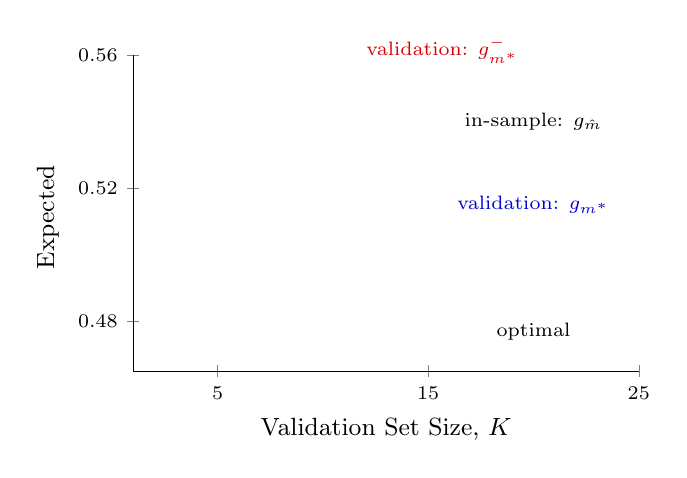
\begin{tikzpicture}
        \begin{axis}[width=8cm, height=5.6cm, xmin=1, xmax=25, ymin=0.465,
            ymax=0.56, axis lines=left, axis line style={-},
            xtick={5,15,25}, ytick={0.48,0.52,0.56},
            yticklabel style={/pgf/number format/fixed,
                /pgf/number format/precision=2},
            tick label style={font=\scriptsize}, label style={font=\small},
            xlabel={Validation Set Size, \(K\)}, ylabel={Expected \(\Eout\)},
            clip=false]
            \valKlines
            \valKred
            \valKblue
            \node[font=\scriptsize, text=red!85!black, anchor=south west] at
                (axis cs:11.6,0.5545) {validation: \(g_{m^*}^-\)};
            \node[font=\scriptsize, anchor=north] at (axis cs:20,0.5455)
                {in-sample: \(g_{\hat{m}}\)};
            \node[font=\scriptsize, text=blue!85!black, anchor=north] at
                (axis cs:20,0.5205) {validation: \(g_{m^*}\)};
            \node[font=\scriptsize, anchor=south] at (axis cs:20,0.4715)
                {optimal};
        \end{axis}
    \end{tikzpicture}
\end{center}

Each curve is the expected \(\Eout\) of the selected hypothesis as the
validation size \(K\) varies. The four strategies are:
\begin{itemize}
    \item \textbf{in-sample} (black, flat): selection with \(\Ein\), which
        does not use \(K\) at all;
    \item \textbf{optimal} (dashed): cheating-selection with \(\Etest\);
    \item \textbf{sub-\(g\)} (red): selection with \(\Eval\), reporting
        \(g_{m^*}^-\);
    \item \textbf{full-\(g\)} (blue): selection with \(\Eval\), reporting
        \(g_{m^*}\). It indeed lies below the red curve, \(\Eout(g_{m^*}) \le
        \Eout(g_{m^*}^-)\), and it beats in-sample selection for every \(K\).
\end{itemize}

\begin{question}
    Why is sub-\(g\) worse than in-sample some time?
\end{question}

Because \(g_{m^*}^-\) is trained on only \(N - K\) examples. Once \(K\) is
large, the loss of training data costs more than the better selection gains;
retraining on all \(N\) examples, as full-\(g\) does, removes that cost.

\subsection{The Dilemma about \texorpdfstring{\(K\)}{K}}

The reasoning of validation is a chain of two approximations:
\[
    \Eout(g) \underset{\text{(small } K)}{\approx} \Eout(g^-)
    \underset{\text{(large } K)}{\approx} \Eval(g^-) .
\]
The two ask for opposite \(K\):
\begin{center}
    \begin{minipage}[c]{0.5\textwidth}
        \begin{itemize}
            \item With large \(K\), every \(\Eval \approx \Eout\), but all
                \(g_m^-\) are much worse than \(g_m\).
            \item With small \(K\), every \(g_m^- \approx g_m\), but \(\Eval\)
                is far from \(\Eout\).
        \end{itemize}
    \end{minipage}%
    \hfill
    \begin{minipage}[c]{0.44\textwidth}
        \centering
        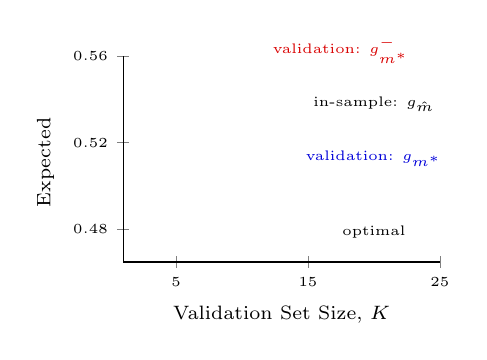
\begin{tikzpicture}
            \begin{axis}[width=5.6cm, height=4.2cm, xmin=1, xmax=25,
                ymin=0.465, ymax=0.56, axis lines=left, axis line style={-},
                xtick={5,15,25}, ytick={0.48,0.52,0.56},
                yticklabel style={/pgf/number format/fixed,
                    /pgf/number format/precision=2},
                tick label style={font=\tiny}, label style={font=\scriptsize},
                xlabel={Validation Set Size, \(K\)},
                ylabel={Expected \(\Eout\)}, clip=false]
                \valKlines
                \valKred
                \valKblue
                \node[font=\tiny, text=red!85!black, anchor=south west] at
                    (axis cs:11.6,0.552) {validation: \(g_{m^*}^-\)};
                \node[font=\tiny, anchor=north] at (axis cs:20,0.5455)
                    {in-sample: \(g_{\hat{m}}\)};
                \node[font=\tiny, text=blue!85!black, anchor=north] at
                    (axis cs:20,0.5205) {validation: \(g_{m^*}\)};
                \node[font=\tiny, anchor=south] at (axis cs:20,0.4715)
                    {optimal};
            \end{axis}
        \end{tikzpicture}
    \end{minipage}
\end{center}

\begin{remark}
    Why both approximations matter: we rank the models by
    \(\Eval(g_m^-)\) but output \(g_{m^*}\), so the chain is what makes
    `smallest \(\Eval(g_m^-)\)' mean `smallest \(\Eout(g_m)\)'. If either link
    breaks, the ranking is wrong and a worse model is picked.
    \begin{itemize}
        \item Small \(K\) breaks the right link: \(\Eval\) is computed on a few
            examples, so its noise can be larger than the true differences
            between models.
        \item Large \(K\) breaks the left link: the ranking is accurate, but it
            ranks the \(g_m^-\) trained on few examples, and the model that is
            best with \(N - K\) examples need not be best with \(N\).
    \end{itemize}
    Both failures raise the \(\Eout\) of the final \(g_{m^*}\): this is the
    U-shape of the blue curve.
\end{remark}

\begin{moral}
    Practical rule of thumb: \(K = \frac{N}{5}\).
\end{moral}

\begin{exercise}[Fun Time]
    For a learning model that takes \(N^2\) seconds of training when using
    \(N\) examples, what is the total amount of seconds needed when running
    the whole validation procedure with \(K = \frac{N}{5}\) on \(25\) such
    models with different parameters to get the final \(g_{m^*}\)?
    \begin{enumerate}[(1)]
        \item \(6N^2\);
        \item \(17N^2\);
        \item \(25N^2\);
        \item \(26N^2\).
    \end{enumerate}
\end{exercise}

\begin{proof}[Reference Answer]
    (2). Each \(g_m^-\) is trained on \(N - K = \frac{4}{5} N\) examples, so to
    get all the \(g_m^-\), we need \(\frac{16}{25} N^2 \cdot 25\) seconds. Then
    to get \(g_{m^*}\), we need another \(N^2\) seconds. So in total we need
    \(17N^2\) seconds.
\end{proof}

\section{Leave-One-Out Cross Validation}\label{sec:loocv}

\source{slides p.13--17}

\subsection{Extreme Case: \texorpdfstring{\(K = 1\)}{K = 1}}

Recall the reasoning of validation:
\[
    \Eout(g) \underset{\text{(small } K)}{\approx} \Eout(g^-)
    \underset{\text{(large } K)}{\approx} \Eval(g^-) .
\]
The first approximation is best at the smallest possible \(K\).
\begin{itemize}
    \item Take \(K = 1\)? Then \(\Dval^{(n)} = \{(\bm{x}_n, y_n)\}\) and
        \[
            \Eval^{(n)}(g_n^-) = \err(g_n^-(\bm{x}_n), y_n) = e_n ,
        \]
        where \(g_n^-\) is learned from all examples except the \(n\)-th.
    \item A single \(e_n\) is a very poor estimate. To make it closer to
        \(\Eout(g)\), average over all possible \(\Eval^{(n)}\), i.e.\ let
        every example take its turn as the validation set.
    \item This gives the \vocab{leave-one-out cross validation} estimate
        \[
            \Eloocv(\mathcal{H}, \mathcal{A}) = \frac{1}{N} \sum_{n=1}^{N} e_n
            = \frac{1}{N} \sum_{n=1}^{N} \err(g_n^-(\bm{x}_n), y_n) .
        \]
        `Cross' because each example is used for training in some rounds and
        for validation in another.
\end{itemize}

\begin{notation}
    Write \(\mathcal{D}_n = \mathcal{D} \setminus \{(\bm{x}_n, y_n)\}\), of size
    \(N - 1\). Then \(g_n^- = \mathcal{A}(\mathcal{D}_n)\): the same model and
    algorithm, trained \(N\) times, each time without one example. The
    subscript now counts the left-out example, not the model as in \(g_m^-\)
    of \autoref{sec:validation}; there is one model and \(N\) hypotheses
    \(g_1^-, \ldots, g_N^-\), and \(g\) itself is \(\mathcal{A}(\mathcal{D})\).
\end{notation}

\begin{moral}
    Hope: \(\Eloocv(\mathcal{H}, \mathcal{A}) \approx \Eout(g)\).
\end{moral}

\subsection{Illustration of Leave-One-Out}

\begin{center}
    \begin{adjustbox}{max width=\textwidth}
        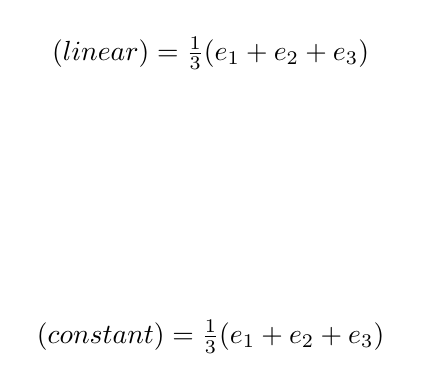
\begin{tikzpicture}
            \loocvRow{linear}
            \node at (4.4,-0.85) {\(\Eloocv(\text{linear}) = \frac{1}{3}(e_1
                + e_2 + e_3)\)};
            \begin{scope}[shift={(0,-3.6)}]
                \loocvRow{constant}
                \node at (4.4,-0.85) {\(\Eloocv(\text{constant}) =
                    \frac{1}{3}(e_1 + e_2 + e_3)\)};
            \end{scope}
        \end{tikzpicture}
    \end{adjustbox}
\end{center}

Three examples, two models. In each panel the red example is left out, the
model is fitted to the other two, and \(e_n\) is the squared length of the red
segment from the left-out example to the fit. The linear model passes exactly
through any two points, but the line through two of them can miss the third
badly, as in the first panel; the constant model is the average height of the
two, and misses all three by moderate amounts.

\begin{question}
    Which one would you choose?
    \[
        m^* = \argmin_{1 \le m \le M} \bigl( E_m =
        \Eloocv(\mathcal{H}_m, \mathcal{A}_m) \bigr)
    \]
\end{question}

\subsection{Theoretical Guarantee of Leave-One-Out Estimate}

Does \(\Eloocv(\mathcal{H}, \mathcal{A})\) say something about \(\Eout(g)\)?
Yes, for the average \(\Eout\) on size-\((N - 1)\) data. Write
\(\overline{\Eout}(N - 1)\) for the expected \(\Eout\) of the hypothesis that
\(\mathcal{A}\) learns from \(N - 1\) examples, and \(\mathcal{D}_n\) for
\(\mathcal{D}\) without \((\bm{x}_n, y_n)\):
\begin{align*}
    \mathop{\mathcal{E}}_{\mathcal{D}} \Eloocv(\mathcal{H}, \mathcal{A}) =
    \mathop{\mathcal{E}}_{\mathcal{D}} \frac{1}{N} \sum_{n=1}^{N} e_n &=
    \frac{1}{N} \sum_{n=1}^{N} \mathop{\mathcal{E}}_{\mathcal{D}} e_n\\
    &= \frac{1}{N} \sum_{n=1}^{N} \mathop{\mathcal{E}}_{\mathcal{D}_n}
    \mathop{\mathcal{E}}_{(\bm{x}_n, y_n)} \err(g_n^-(\bm{x}_n), y_n)\\
    &= \frac{1}{N} \sum_{n=1}^{N} \mathop{\mathcal{E}}_{\mathcal{D}_n}
    \Eout(g_n^-)\\
    &= \frac{1}{N} \sum_{n=1}^{N} \overline{\Eout}(N - 1) =
    \overline{\Eout}(N - 1) .
\end{align*}
Line by line:
\begin{itemize}
    \item The first equality is linearity of expectation.
    \item The second splits \(\mathcal{D}\) into \(\mathcal{D}_n\) and the
        left-out example. They are independent, and \(g_n^-\) depends only on
        \(\mathcal{D}_n\).
    \item The third holds because, for a fixed \(g_n^-\), the expected error
        on a fresh example \((\bm{x}_n, y_n) \sim P\) is exactly
        \(\Eout(g_n^-)\).
    \item The last holds because each \(\mathcal{D}_n\) is just an iid data
        set of size \(N - 1\), so every term is the same
        \(\overline{\Eout}(N - 1)\).
\end{itemize}

\begin{moral}
    The expected \(\Eloocv(\mathcal{H}, \mathcal{A})\) says something about
    the expected \(\Eout(g^-)\), often called an `almost unbiased estimate
    of \(\Eout(g)\)'.
\end{moral}

`Almost' because the left side matches the learning curve at \(N - 1\), not
at \(N\), and the two differ by one example only.

\begin{remark}
    This says \(\Eloocv\) is an honest estimate, not that it is small.
    \begin{itemize}
        \item A bad model gets a large \(\Eloocv\), and that is the right
            answer: the estimate reports \(\Eout\), it does not lower it.
        \item Small \(\Eout\) comes from the selection: computing
            \(\Eloocv(\mathcal{H}_m, \mathcal{A}_m)\) for each of the \(M\)
            models and taking the smallest picks the model whose \(\Eout\) is
            estimated to be lowest, as \(\Eval\) did in
            \autoref{sec:validation}.
        \item If even the best \(\Eloocv\) is large, no candidate is good
            enough, and a better model or more data has to come from outside
            validation.
    \end{itemize}
    The guarantee is also only an expectation over \(\mathcal{D}\): on one
    data set \(\Eloocv\) can still miss, a weakness taken up in
    \autoref{sec:vfold}.
\end{remark}

\subsection{Leave-One-Out in Practice}

The handwritten-digit task of \autoref{sec:nonlin-transform}: classify `1'
versus `not 1' from the two features average intensity and symmetry. The
model is a polynomial transform followed by a linear classifier, and the
number of features used is the knob to be selected.

\begin{notation}
    Write \(\bm{x} = (x_1, x_2)\) for (intensity, symmetry). The full
    \(5\)th-order transform lists its terms by degree,
    \[
        \bm{\Phi}(\bm{x}) = (1, x_1, x_2, x_1^2, x_1 x_2, x_2^2, x_1^3,
        \ldots, x_1 x_2^4, x_2^5),
    \]
    with \(20\) features besides the constant. `\(\#\) features used \(= k\)'
    is the model \(\mathcal{H}_k\) that keeps only the constant and the first
    \(k\) of them: \(k = 2\) is linear, \(k = 5\) is the full quadratic, \(k =
    20\) the full quintic. The models are nested, \(\mathcal{H}_1 \subset
    \mathcal{H}_2 \subset \cdots \subset \mathcal{H}_{20}\), so moving right
    on the horizontal axis means a more complex model. This setup follows
    \emph{Learning from Data} (Abu-Mostafa et al.), where the plot comes from.
\end{notation}

\begin{center}
    \begin{tikzpicture}
        \node[anchor=south] at (0,0)
            {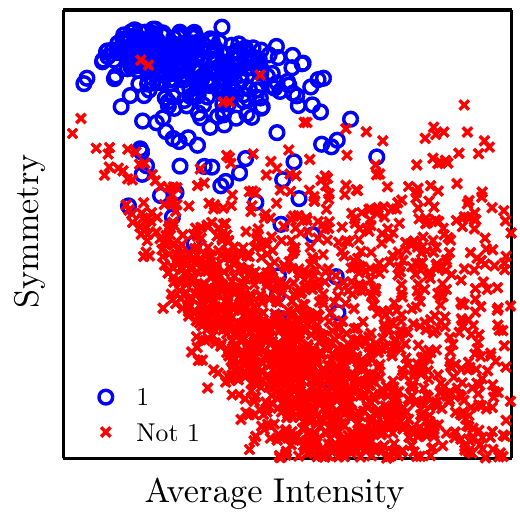
\includegraphics[width=4.6cm]{Figures/loocv_digits_data.png}};
        \node[anchor=south] at (4.9,0)
            {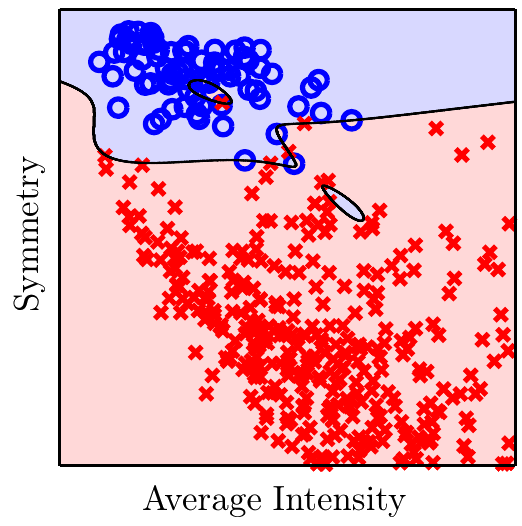
\includegraphics[width=4.6cm]{Figures/loocv_digits_ein.png}};
        \node[anchor=south] at (9.8,0)
            {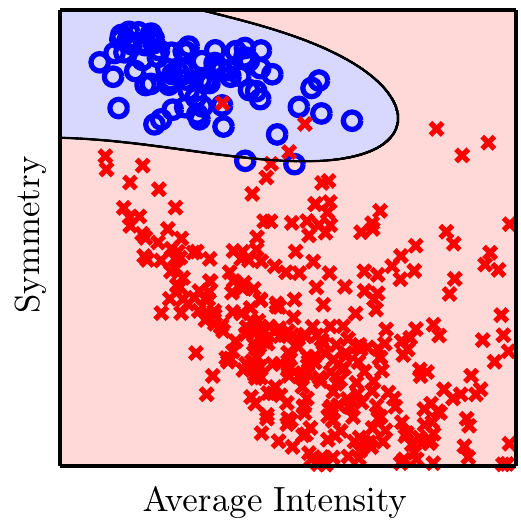
\includegraphics[width=4.6cm]{Figures/loocv_digits_eloocv.png}};
        \node[anchor=north] at (4.9,0) {select by \(\Ein\)};
        \node[anchor=north] at (9.8,0) {select by \(\Eloocv\)};
    \end{tikzpicture}
\end{center}

\begin{center}
    \begin{tikzpicture}
        \begin{axis}[width=7cm, height=5.2cm, xmin=2, xmax=20, ymin=0,
            ymax=0.03, axis lines=left, axis line style={-},
            xtick={5,10,15,20}, ytick={0.01,0.02,0.03},
            yticklabel style={/pgf/number format/fixed,
                /pgf/number format/precision=2},
            tick label style={font=\scriptsize}, label style={font=\small},
            xlabel={\# Features Used}, ylabel={Error}, scaled y ticks=false,
            clip=false]
            \loocvEout
            \loocvEcv
            \loocvEin
            \node[font=\scriptsize, text=red!85!black, anchor=south] at
                (axis cs:9,0.0175) {\(\Eout\)};
            \node[font=\scriptsize, anchor=west] at (axis cs:12.4,0.0145)
                {\(\Ecv\)};
            \node[font=\scriptsize, text=blue!85!black, anchor=south] at
                (axis cs:18.5,0.0022) {\(\Ein\)};
        \end{axis}
    \end{tikzpicture}
\end{center}

The left scatter is the data, blue circles for `1' and red crosses for `not
1'. \(\Ein\) (blue curve) keeps falling as features are added, so selecting by
\(\Ein\) takes the most features and returns the twisted boundary of the
middle plot, with small islands carved around single examples. The
leave-one-out estimate (black curve, labelled \(\Ecv\)) follows the shape of
\(\Eout\) (red) much more closely, is smallest at around five to seven
features, and selects the smooth boundary of the right plot.

\begin{moral}
    \(\Eloocv\) is much better than \(\Ein\).
\end{moral}

\begin{exercise}[Fun Time]
    Consider three examples \((\bm{x}_1, y_1)\), \((\bm{x}_2, y_2)\),
    \((\bm{x}_3, y_3)\) with \(y_1 = 1\), \(y_2 = 5\), \(y_3 = 7\). If we use
    \(\Eloocv\) to estimate the performance of a learning algorithm that
    predicts with the average \(y\) value of the data set --- the optimal
    constant prediction with respect to the squared error --- what is
    \(\Eloocv\) (squared error) of the algorithm?
    \begin{enumerate}[(1)]
        \item \(0\);
        \item \(\frac{56}{9}\);
        \item \(\frac{60}{9}\);
        \item \(14\).
    \end{enumerate}
\end{exercise}

\begin{proof}[Reference Answer]
    (4). The algorithm ignores \(\bm{x}\): trained on any data set, it returns
    the constant hypothesis equal to the average \(y\) of that set. So each
    \(g_n^- = \mathcal{A}(\mathcal{D}_n)\) is the average of the two \(y\)'s
    left after removing \((\bm{x}_n, y_n)\), and \(e_n\) is its squared error on
    the removed \(y_n\):
    \begin{center}
        \solidrules
        \begin{tabular}{c|c|c|c}
            \toprule
            \(n\) & \(\mathcal{D}_n\) keeps & \(g_n^-(\bm{x})\) &
            \(e_n = (y_n - g_n^-(\bm{x}_n))^2\) \\
            \midrule
            \(1\) & \(y_2 = 5,\ y_3 = 7\) & \(\frac{5 + 7}{2} = 6\) &
            \((1 - 6)^2 = 25\) \\
            \(2\) & \(y_1 = 1,\ y_3 = 7\) & \(\frac{1 + 7}{2} = 4\) &
            \((5 - 4)^2 = 1\) \\
            \(3\) & \(y_1 = 1,\ y_2 = 5\) & \(\frac{1 + 5}{2} = 3\) &
            \((7 - 3)^2 = 16\) \\
            \bottomrule
        \end{tabular}
    \end{center}
    Then \(\Eloocv = \frac{1}{3}(25 + 1 + 16) = 14\). The final hypothesis
    \(g = \mathcal{A}(\mathcal{D})\) is the constant \(\frac{1 + 5 + 7}{3} =
    \frac{13}{3}\), but it plays no part in computing \(\Eloocv\).
\end{proof}

\section{\texorpdfstring{\(V\)}{V}-Fold Cross Validation}\label{sec:vfold}

\source{slides p.18--21}

\subsection{Disadvantages of Leave-One-Out Estimate}

\paragraph{Computation.}
\[
    \Eloocv(\mathcal{H}, \mathcal{A}) = \frac{1}{N} \sum_{n=1}^{N} e_n =
    \frac{1}{N} \sum_{n=1}^{N} \err(g_n^-(\bm{x}_n), y_n)
\]
\begin{itemize}
    \item Each \(e_n\) needs its own \(g_n^-\), so there are \(N\)
        `additional' trainings per model, which is not always feasible in
        practice.
    \item The exception is a `special case' such as the analytic solution of
        linear regression, where all \(N\) leave-one-out errors can be
        computed from one fit.
\end{itemize}

\paragraph{Stability --- due to variance of single-point estimates.}

\begin{center}
    \begin{tikzpicture}
        \begin{axis}[width=6.4cm, height=4.6cm, xmin=2, xmax=20, ymin=0,
            ymax=0.03, axis lines=left, axis line style={-},
            xtick={5,10,15,20}, ytick={0.01,0.02,0.03},
            yticklabel style={/pgf/number format/fixed,
                /pgf/number format/precision=2},
            tick label style={font=\scriptsize}, label style={font=\small},
            xlabel={\# Features Used}, ylabel={Error}, scaled y ticks=false,
            clip=false]
            \loocvEout
            \loocvEcv
            \loocvEin
            \node[font=\scriptsize, text=red!85!black, anchor=south] at
                (axis cs:9,0.0175) {\(\Eout\)};
            \node[font=\scriptsize, anchor=west] at (axis cs:12.4,0.0145)
                {\(\Ecv\)};
            \node[font=\scriptsize, text=blue!85!black, anchor=south] at
                (axis cs:18.5,0.0022) {\(\Ein\)};
        \end{axis}
    \end{tikzpicture}
\end{center}

The same curves as before. Each \(e_n\) is the error on a single example, so
it jumps between \(0\) and \(1\) for classification, and the average of such
jumpy terms is itself jumpy: the black curve zigzags up and down from one
number of features to the next, where \(\Eout\) is smooth.

\begin{moral}
    \(\Eloocv\): not often used practically.
\end{moral}

\subsection{\texorpdfstring{\(V\)}{V}-fold Cross Validation}

\begin{question}
    How to decrease the computation need for cross validation?
\end{question}

\begin{itemize}
    \item The essence of leave-one-out cross validation is to partition
        \(\mathcal{D}\) into \(N\) parts, and in order take \(N - 1\) of them
        for training and \(1\) for validation.
    \item \vocab{\(V\)-fold cross validation} instead makes a random partition
        of \(\mathcal{D}\) into \(V\) equal parts,
        \begin{center}
            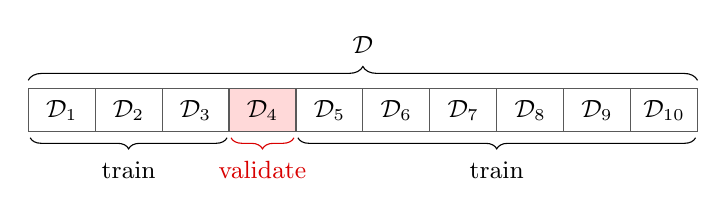
\begin{tikzpicture}[font=\small]
                \foreach \i/\c in {1/white, 2/white, 3/white, 4/red!15,
                        5/white, 6/white, 7/white, 8/white, 9/white,
                        10/white}{
                    \node[draw=black!65, minimum width=0.85cm,
                        minimum height=0.55cm, inner sep=0pt, fill=\c]
                        at ({0.85*\i},0) {\(\mathcal{D}_{\i}\)};}
                \draw[decorate, decoration={brace, amplitude=5pt}]
                    (0.425,0.38) -- (8.925,0.38)
                    node[midway, above=6pt] {\(\mathcal{D}\)};
                \draw[decorate, decoration={brace, mirror, amplitude=4pt}]
                    (0.45,-0.35) -- (2.95,-0.35)
                    node[midway, below=5pt] {train};
                \draw[decorate, decoration={brace, mirror, amplitude=4pt},
                    red!85!black] (3.0,-0.35) -- (3.8,-0.35)
                    node[midway, below=5pt] {validate};
                \draw[decorate, decoration={brace, mirror, amplitude=4pt}]
                    (3.85,-0.35) -- (8.9,-0.35)
                    node[midway, below=5pt] {train};
            \end{tikzpicture}
        \end{center}
        and in order takes \(V - 1\) of them for training and \(1\) for
        validation, here the fourth one. Averaging the \(V\) validation errors
        gives
        \[
            \Ecv(\mathcal{H}, \mathcal{A}) = \frac{1}{V} \sum_{v=1}^{V}
            \Eval^{(v)}(g_v^-) .
        \]
    \item Selection is then by \(\Ecv\):
        \[
            m^* = \argmin_{1 \le m \le M} \bigl( E_m = \Ecv(\mathcal{H}_m,
            \mathcal{A}_m) \bigr) .
        \]
\end{itemize}

Leave-one-out is the special case \(V = N\). A smaller \(V\) needs only \(V\)
trainings per model, and each \(\Eval^{(v)}\) averages over \(N / V\)
examples instead of one, which also tames the zigzag.

\begin{moral}
    Practical rule of thumb: \(V = 10\).
\end{moral}

\subsection{Final Words on Validation}

\paragraph{`Selecting' a validation tool.}
\begin{itemize}
    \item \(V\)-fold is generally preferred over single validation if the
        computation allows it, because every example is used for validation
        once instead of only the \(K\) set aside.
    \item 5-fold or 10-fold generally works well, so it is not necessary to
        trade \(V\)-fold for the much more expensive leave-one-out.
\end{itemize}

\paragraph{Nature of validation.}
\begin{itemize}
    \item All training models select among hypotheses: \(\mathcal{A}_m\)
        picks \(g_m\) from \(\mathcal{H}_m\).
    \item All validation schemes select among finalists: they pick one of the
        \(M\) already-learned \(g_m^-\).
    \item All testing methods just evaluate: they make no choice at all.
\end{itemize}
Validation is still a selection, so it is still contaminated by a little
optimism. That is, validation is more optimistic than testing.

\begin{moral}
    Do not fool yourself and others :-) Report the test result, not the best
    validation result.
\end{moral}

\begin{exercise}[Fun Time]
    For a learning model that takes \(N^2\) seconds of training when using
    \(N\) examples, what is the total amount of seconds needed when running
    10-fold cross validation on \(25\) such models with different parameters
    to get the final \(g_{m^*}\)?
    \begin{enumerate}[(1)]
        \item \(\frac{47}{2} N^2\);
        \item \(47N^2\);
        \item \(\frac{407}{2} N^2\);
        \item \(407N^2\).
    \end{enumerate}
\end{exercise}

\begin{proof}[Reference Answer]
    (3). Each fold trains on \(\frac{9}{10} N\) examples, so to get all the
    \(\Ecv\), we need \(\frac{81}{100} N^2 \cdot 10 \cdot 25\) seconds. Then
    to get \(g_{m^*}\), we need another \(N^2\) seconds. So in total we need
    \(\frac{407}{2} N^2\) seconds.
\end{proof}

\hrulebar

\subsection*{Summary}

\begin{description}
    \item[Model Selection Problem] dangerous by \(\Ein\) and dishonest by
        \(\Etest\).
    \item[Validation] select with \(\Eval(\mathcal{A}_m(\Dtrain))\) while
        returning \(\mathcal{A}_{m^*}(\mathcal{D})\).
    \item[Leave-One-Out Cross Validation] huge computation for almost unbiased
        estimate.
    \item[\(V\)-Fold Cross Validation] reasonable computation and performance.
\end{description}

Validation (crossly) reserves data to simulate the testing procedure, and it
answers how to choose \(\lambda\) and every other knob of a learning model.
Next: something `up my sleeve' --- three principles that summarize what to
keep in mind when learning.
